\FloatBarrier
\section{Manufacturing, test, yield and reliability}\label{sec:mfg}

\subsection{Wafer flow and mask set}
The compute die uses 79 masks: 18 EUV for the critical front-end and middle-of-line layers, 61 DUV
for the remainder, including the backside power layers. The two L3 dies are fabricated in a
6 nm-class process on the same 300 mm line and hybrid-bonded after both wafers have been tested.
The HBM stacks are purchased as known-good die from a memory vendor and assembled on the
interposer with the usual mass-reflow process.

Wafer sort is a two-touch flow. The first touch checks the large SRAM arrays and the tile
datapath with a march test and a scan-based structural test; the second runs at-speed capture on
the cluster clock domains and a loopback test on the SerDes. The tile array is regular enough that
a single failed AVT can be disabled and the die sold as a 56- or 48-tile part, which recovers
roughly 6\% of otherwise-lost die.

\subsection{Yield}
The die is 287.6 mm$^2$ and the defect density assumption is 0.09 cm$^{-2}$, which gives a Murphy
yield of \ACYieldDie\%. A 300 mm wafer yields 209 gross dies and 162 good ones. The L3 dies are
small enough (42 mm$^2$) to yield above 95\%, and the known-good-die flow removes them from the
compute-die yield equation. The compound package yield, including assembly and test, is 88\%.

\begin{table}[t]
\centering\small
\caption{Cost model at the 100k-unit volume. The card bill of materials excludes the heatsink,
which is sold as part of the card.}
\label{tab:cost}
\begin{tabular}{@{}lrr@{}}
\toprule
Item & Unit cost & Share\\
\midrule
Compute die (162 good per wafer, \$24k wafer) & \$148 & 32\%\\
Two L3 dies & \$24 & 5\%\\
Two HBM3E stacks (48 GB) & \$84 & 18\%\\
Interposer and assembly & \$55 & 12\%\\
Test and burn-in & \$88 & 19\%\\
PCB and cooling & \$65 & 14\%\\
\midrule
Card bill of materials & \$464 & 100\%\\
Selling price & \$1{,}499 & \\
Gross margin & 69\% & \\
\bottomrule
\end{tabular}
\end{table}

\subsection{Test and qualification}
The test plan has five layers: structural scan (98.7\% stuck-at and 94\% transition coverage),
memory BIST on the 1.41 Gbit of SRAM, at-speed functional test of the AVT datapath with a
pre-computed signature, SerDes and HBM loopback, and a system-level test that runs a small ensemble
through the driver stack. Burn-in is 24 hours at 125 $^\circ$C and 1.1 V, followed by a 100\%
at-speed retest; the outgoing defect rate target is below 200 DPPM.

Qualification follows JEDEC-style stress: 1,000 hours of high-temperature operating life at
125 $^\circ$C, 1,000 temperature cycles between $-40$ and $+125$ $^\circ$C, biased HAST, and
package-level drop and vibration tests for the dual-slot card. The card is a passive, fan-cooled
device, so there is no battery or moving-part qualification beyond the fan itself.

\subsection{Reliability}
Three mechanisms dominate. Electromigration in the global power grid is kept below 1\% of the
Black-equation lifetime at 105 $^\circ$C; the backside power layers help because they carry current
in wider, cooler metal. Gate-oxide wear-out is modelled with a Weibull distribution whose
$\beta=1.6$ and whose scale puts the first 1 ppm of failures beyond 47 years at 1.05 V. Soft errors
in the 1.41 Gbit of SRAM are the largest single contributor to the failure budget: SEC-DED reduces
an expected 2.8 M FIT of correctable events to about 280 FIT of uncorrectable ones, and a 24-hour
scrub keeps the probability of a double-bit accumulation negligible.

\begin{figure}[t]
\centering
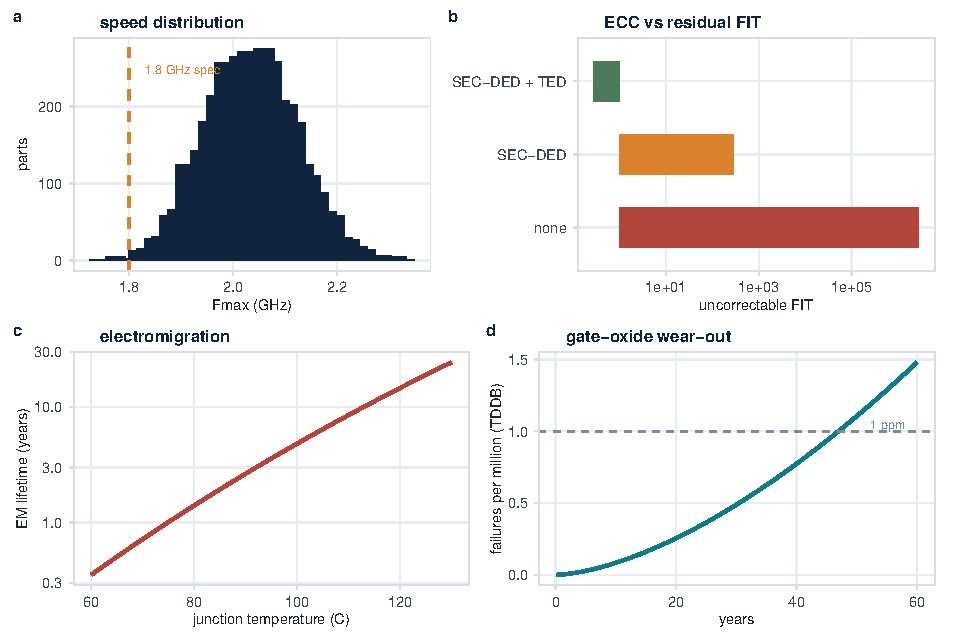
\includegraphics[width=\linewidth]{fig25_reliability}
\caption{Reliability. (a) Fmax distribution from 4,000 Monte-Carlo samples; 99.7\% of parts meet
1.8 GHz and 65\% reach 2.0 GHz. (b) Correctable and residual FIT against ECC scheme. (c)
Electromigration lifetime against junction temperature at 1.5 MA/cm$^2$. (d) Gate-oxide wear-out,
failures per million against years.}
\label{fig:reliability}
\end{figure}

\begin{figure}[t]
\centering
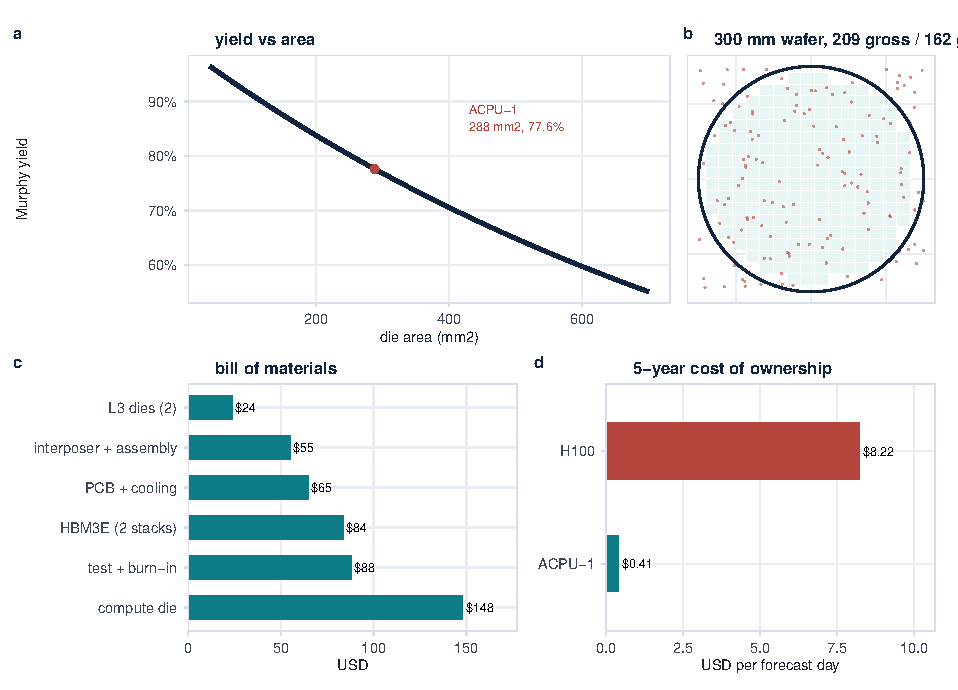
\includegraphics[width=\linewidth]{fig22_yield}
\caption{Yield and cost. (a) Murphy yield against die area with the \ac{1} point marked. (b) Wafer
map with 140 simulated defects and 209 gross dies. (c) Bill of materials. (d) Five-year cost of
ownership per forecast day, including capex and electricity at \$0.12/kWh.}
\label{fig:yield}
\end{figure}

\subsection{Cost of ownership}
Table~\ref{tab:cost} and Fig.~\ref{fig:yield} give the economics. A card costs \$464 to build and
sells for \$1,499, a 69\% gross margin that is normal for a low-volume accelerator. The interesting
number is the five-year cost per forecast day: \$0.41 for \ac{1} against \$8.22 for an H100, where
the difference is almost entirely capital amortisation rather than electricity. The H100 is a
general machine priced for a much larger market; \ac{1} is cheap because it is small, not because
it is subsidised.
